\documentclass[]{article}
\usepackage{amsmath}
\usepackage{amsfonts}
\usepackage{amssymb}
\usepackage{algorithmic}
\usepackage{algorithm}
\usepackage{tikz}
\usepackage{graphicx}
\usepackage{mdframed}
\usepackage{paralist}
\usepackage{listings}

\definecolor{dkgreen}{rgb}{0,0.6,0}
\definecolor{gray}{rgb}{0.5,0.5,0.5}

\lstset{
  language=Python,
  breaklines=true,
  showstringspaces=false,
  frame=single,
  aboveskip=3mm,
  belowskip=3mm,
  columns=flexible,
  basicstyle={\small\ttfamily},
  numbers=none,
  numberstyle=\tiny\color{gray},
  keywordstyle=\color{blue},
  commentstyle=\color{gray},
  stringstyle=\color{dkgreen},
  breakatwhitespace=true,
  tabsize=3
}

\title{CAGD - Homework 3}
\author{Josefine St{\aa}l \& Erik Ackzell}

\begin{document}

\maketitle
\section*{Task 3}
In this task we implement a method to check whether a real number is in an interval with full support, given a knot sequence, a degree of the spline basis and the number itself. The code can be seen in Appendix I. \\
We tried our code for three different knot sequences, $k_1=(0, 0, 1, 1)$, $k_2=(0, 0, 0, 1, 1, 1)$ and $k_3=(0, 0, 0, 0.3, 0.5, 0.6, 1, 1, 1)$, all with quadratic splines. For each of the scenarios, we tested our code with the real numbers $\{0.12, 0.24, 0.4, 0.53, 0.78, 0.8\}$.
\begin{itemize}
	\item For $k_1$, we found that all points were in intervals \textbf{without} full support.
	\item For $k_2$, we found that all points were in intervals \textbf{with} full support.
	\item For $k_3$, we found that all points were in intervals \textbf{with} full support.
\end{itemize}
The results were as expected, as an interval has full support when using quadratic splines, if there are 3 or more knots to the left of the left point of the interval as well as to the right of the right point of the interval.

\section*{Task 4}
In this task we plot the spline curve with knots $\{0, 0, 0, 0.3, 0.5, 0.5, 0.6, 1, 1, 1\}$ and control points 
$\{(0, 0), (3, 4), (7, 5), (9, 2), (13, 1), (10, -1), (7, -1)\}$. We do this by using the definition of the spline, $C(u)=\sum_{i=0}^{m}d_iN_i^n(u)$, where $d_i$ are the control points and $N_i^n$ are the spline basis functions. The methods implemented in the previous tasks are used to achieve this. \\
\\
The plot can be seen below and the code can be seen in Appendix I. As the number of knots is 10 and the number of control points is 7, the degree of the curve is $10 - 1 - 7 = 2$. Thus, the kink at the knot $0.5$ is expected, as the curve is only $2-2=0$ times continuous at a knot of multiplicity $2$.
\begin{figure}[h!]
	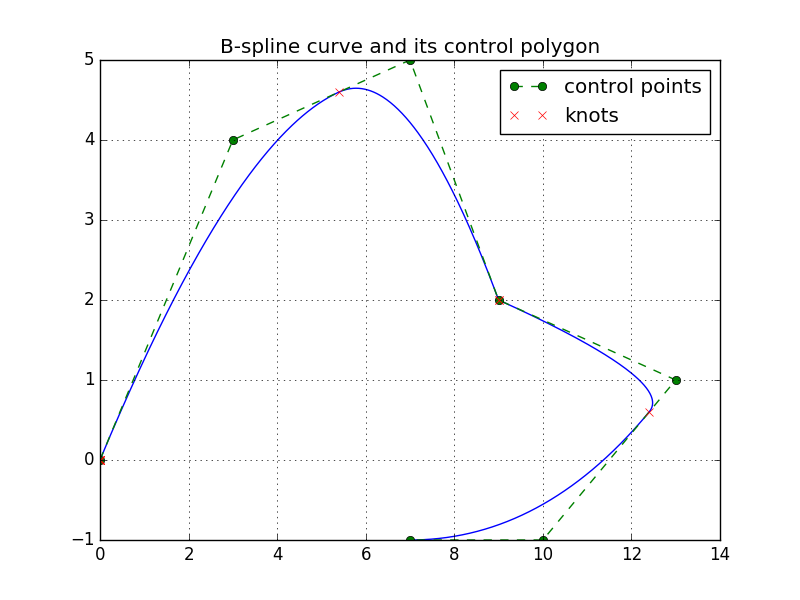
\includegraphics[scale=0.6]{bspline}
\end{figure}


\newpage
\section*{Appendix I}
\lstinputlisting[lastline=87]{bsplines.py}

\end{document}
